\documentclass[border=4pt]{standalone}
\usepackage{fontspec}
\usepackage{amsmath}
\usepackage{unicode-math}
\setmainfont{Latin Modern Roman}
\setmathfont{Latin Modern Math}
\usepackage{pgfplots}
\usepackage{pgfplotstable}
\pgfplotsset{compat=1.18}
\usepackage{tkz-euclide}
\usetikzlibrary{arrows.meta,calc,angles,quotes,patterns,3d,backgrounds}
\definecolor{ink}{HTML}{123428}
\definecolor{asy}{HTML}{475569}
\definecolor{mint}{HTML}{86e0bd}
\tikzset{asym/.style={asy, line width=0.9pt, dash pattern=on 5pt off 3.5pt},
         guide/.style={gray!70, line width=0.6pt, densely dotted},
         dot/.style={circle, inner sep=0pt, minimum size=5pt, draw=white, line width=0.5pt},
         odot/.style={circle, inner sep=0pt, minimum size=5.5pt, fill=white, line width=1pt},
         lab/.style={font=\footnotesize, inner sep=1.5pt, text=ink}}
\begin{document}
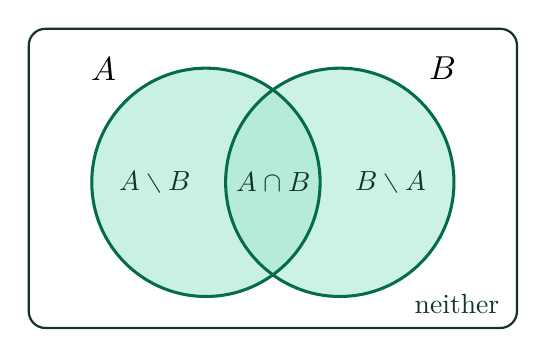
\begin{tikzpicture}[x=1cm, y=1cm]
\def\A{(-0.85,0) circle (1.45)}
\def\B{(0.85,0) circle (1.45)}
\fill[mint!45] \A; \fill[mint!70, fill opacity=0.6] \B;
\draw[ink, line width=0.8pt, rounded corners=6pt] (-3.1,-1.85) rectangle (3.1,1.95);
\draw[draw={rgb,255:red,4;green,107;blue,77}, line width=1.1pt] \A; \draw[draw={rgb,255:red,4;green,107;blue,77}, line width=1.1pt] \B;
\node[font=\large] at (-2.15,1.45) {$A$};
\node[font=\large] at (2.15,1.45) {$B$};
\node[font=\normalsize, text=ink] at (-1.5,0) {$A\setminus B$};
\node[font=\normalsize, text=ink] at (0,0) {$A\cap B$};
\node[font=\normalsize, text=ink] at (1.5,0) {$B\setminus A$};
\node[font=\normalsize, text=ink, anchor=south east] at (3.0,-1.8) {neither};
\end{tikzpicture}
\end{document}
